\documentclass{standalone}
\usepackage{tikz}
\usetikzlibrary{patterns, positioning}

\begin{document}
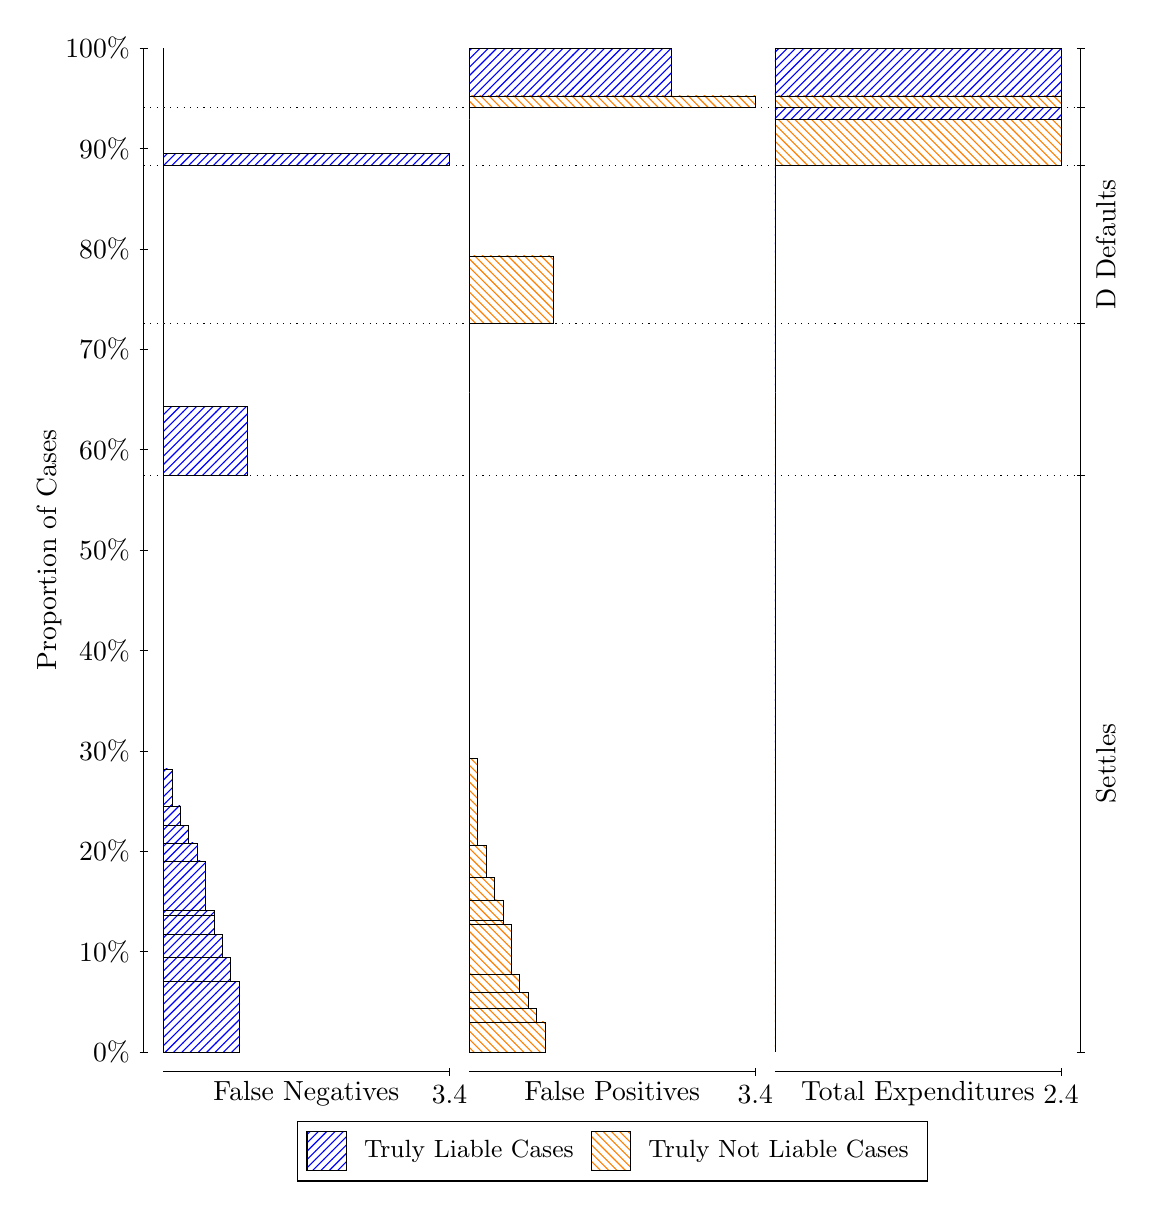
\begin{tikzpicture}
\draw[black, very thin] (1.5,1.75) -- (1.5,14.5);
\node[rotate=90, anchor=center] at (0.3, 8.125) {Proportion of Cases};
\draw[black, very thin] (1.45,1.75) -- (1.55,1.75);
\node[anchor=east] at (1.45, 1.75) {0\%};
\draw[black, very thin] (1.45,3.025) -- (1.55,3.025);
\node[anchor=east] at (1.45, 3.025) {10\%};
\draw[black, very thin] (1.45,4.3) -- (1.55,4.3);
\node[anchor=east] at (1.45, 4.3) {20\%};
\draw[black, very thin] (1.45,5.575) -- (1.55,5.575);
\node[anchor=east] at (1.45, 5.575) {30\%};
\draw[black, very thin] (1.45,6.85) -- (1.55,6.85);
\node[anchor=east] at (1.45, 6.85) {40\%};
\draw[black, very thin] (1.45,8.125) -- (1.55,8.125);
\node[anchor=east] at (1.45, 8.125) {50\%};
\draw[black, very thin] (1.45,9.4) -- (1.55,9.4);
\node[anchor=east] at (1.45, 9.4) {60\%};
\draw[black, very thin] (1.45,10.675) -- (1.55,10.675);
\node[anchor=east] at (1.45, 10.675) {70\%};
\draw[black, very thin] (1.45,11.95) -- (1.55,11.95);
\node[anchor=east] at (1.45, 11.95) {80\%};
\draw[black, very thin] (1.45,13.225) -- (1.55,13.225);
\node[anchor=east] at (1.45, 13.225) {90\%};
\draw[black, very thin] (1.45,14.5) -- (1.55,14.5);
\node[anchor=east] at (1.45, 14.5) {100\%};

\draw[black, very thin] (13.4,1.75) -- (13.4,14.5);
\draw[black, very thin] (13.35,1.75) -- (13.45,1.75);
\node[anchor=west] at (13.35, 1.75) {};
\draw[black, very thin] (13.35,9.0764) -- (13.45,9.0764);
\node[anchor=west] at (13.35, 9.0764) {};
\draw[black, very thin] (13.35,11.002) -- (13.45,11.002);
\node[anchor=west] at (13.35, 11.002) {};
\draw[black, very thin] (13.35,13.008) -- (13.45,13.008);
\node[anchor=west] at (13.35, 13.008) {};
\draw[black, very thin] (13.35,13.742) -- (13.45,13.742);
\node[anchor=west] at (13.35, 13.742) {};
\draw[black, very thin] (13.35,14.5) -- (13.45,14.5);
\node[anchor=west] at (13.35, 14.5) {};

\draw[black, very thin, pattern color=blue, pattern=north east lines] (1.75,1.75) rectangle (2.7118,2.6487);
\draw[black, very thin, pattern color=blue, pattern=north east lines] (1.75,2.6487) rectangle (2.6049,2.9506);
\draw[black, very thin, pattern color=blue, pattern=north east lines] (1.75,2.9506) rectangle (2.498,3.2391);
\draw[black, very thin, pattern color=blue, pattern=north east lines] (1.75,3.2391) rectangle (2.3912,3.4871);
\draw[black, very thin, pattern color=blue, pattern=north east lines] (1.75,3.4871) rectangle (2.3912,3.5504);
\draw[black, very thin, pattern color=blue, pattern=north east lines] (1.75,3.5504) rectangle (2.2843,4.1759);
\draw[black, very thin, pattern color=blue, pattern=north east lines] (1.75,4.1759) rectangle (2.1775,4.4063);
\draw[black, very thin, pattern color=blue, pattern=north east lines] (1.75,4.4063) rectangle (2.0706,4.6306);
\draw[black, very thin, pattern color=blue, pattern=north east lines] (1.75,4.6306) rectangle (1.9637,4.8765);
\draw[black, very thin, pattern color=blue, pattern=north east lines] (1.75,4.8765) rectangle (1.8569,5.3452);
\draw[black, very thin, pattern color=orange, pattern=north west lines] (1.75,5.3452) rectangle (1.75,9.0764);
\draw[black, very thin, pattern color=blue, pattern=north east lines] (1.75,9.0764) rectangle (2.8186,9.9497);
\draw[black, very thin, pattern color=orange, pattern=north west lines] (1.75,9.9497) rectangle (1.75,11.002);
\draw[black, very thin, pattern color=orange, pattern=north west lines] (1.75,11.002) rectangle (1.75,11.86);
\draw[black, very thin, pattern color=blue, pattern=north east lines] (1.75,11.86) rectangle (1.75,13.008);
\draw[black, very thin, pattern color=blue, pattern=north east lines] (1.75,13.008) rectangle (5.3833,13.158);
\draw[black, very thin, pattern color=orange, pattern=north west lines] (1.75,13.158) rectangle (1.75,13.742);
\draw[black, very thin, pattern color=orange, pattern=north west lines] (1.75,13.742) rectangle (1.75,13.892);
\draw[black, very thin, pattern color=blue, pattern=north east lines] (1.75,13.892) rectangle (1.75,14.5);
\draw[black, very thin, pattern color=orange, pattern=north west lines] (5.6333,1.75) rectangle (6.5951,2.1332);
\draw[black, very thin, pattern color=orange, pattern=north west lines] (5.6333,2.1332) rectangle (6.4882,2.3085);
\draw[black, very thin, pattern color=orange, pattern=north west lines] (5.6333,2.3085) rectangle (6.3814,2.5035);
\draw[black, very thin, pattern color=orange, pattern=north west lines] (5.6333,2.5035) rectangle (6.2745,2.7324);
\draw[black, very thin, pattern color=orange, pattern=north west lines] (5.6333,2.7324) rectangle (6.1676,3.3725);
\draw[black, very thin, pattern color=orange, pattern=north west lines] (5.6333,3.3725) rectangle (6.0608,3.4251);
\draw[black, very thin, pattern color=orange, pattern=north west lines] (5.6333,3.4251) rectangle (6.0608,3.6822);
\draw[black, very thin, pattern color=orange, pattern=north west lines] (5.6333,3.6822) rectangle (5.9539,3.9687);
\draw[black, very thin, pattern color=orange, pattern=north west lines] (5.6333,3.9687) rectangle (5.8471,4.3756);
\draw[black, very thin, pattern color=orange, pattern=north west lines] (5.6333,4.3756) rectangle (5.7402,5.4812);
\draw[black, very thin, pattern color=blue, pattern=north east lines] (5.6333,5.4812) rectangle (5.6333,9.0764);
\draw[black, very thin, pattern color=orange, pattern=north west lines] (5.6333,9.0764) rectangle (5.6333,10.128);
\draw[black, very thin, pattern color=blue, pattern=north east lines] (5.6333,10.128) rectangle (5.6333,11.002);
\draw[black, very thin, pattern color=orange, pattern=north west lines] (5.6333,11.002) rectangle (6.702,11.86);
\draw[black, very thin, pattern color=blue, pattern=north east lines] (5.6333,11.86) rectangle (5.6333,13.008);
\draw[black, very thin, pattern color=orange, pattern=north west lines] (5.6333,13.008) rectangle (5.6333,13.591);
\draw[black, very thin, pattern color=blue, pattern=north east lines] (5.6333,13.591) rectangle (5.6333,13.742);
\draw[black, very thin, pattern color=orange, pattern=north west lines] (5.6333,13.742) rectangle (9.2667,13.892);
\draw[black, very thin, pattern color=blue, pattern=north east lines] (5.6333,13.892) rectangle (8.198,14.5);
\draw[black, very thin, pattern color=orange, pattern=north west lines] (9.5167,1.75) rectangle (9.5167,5.4812);
\draw[black, very thin, pattern color=blue, pattern=north east lines] (9.5167,5.4812) rectangle (9.5167,9.0764);
\draw[black, very thin, pattern color=orange, pattern=north west lines] (9.5167,9.0764) rectangle (9.5167,10.128);
\draw[black, very thin, pattern color=blue, pattern=north east lines] (9.5167,10.128) rectangle (9.5167,11.002);
\draw[black, very thin, pattern color=orange, pattern=north west lines] (9.5167,11.002) rectangle (9.5167,11.86);
\draw[black, very thin, pattern color=blue, pattern=north east lines] (9.5167,11.86) rectangle (9.5167,13.008);
\draw[black, very thin, pattern color=orange, pattern=north west lines] (9.5167,13.008) rectangle (13.15,13.591);
\draw[black, very thin, pattern color=blue, pattern=north east lines] (9.5167,13.591) rectangle (13.15,13.742);
\draw[black, very thin, pattern color=orange, pattern=north west lines] (9.5167,13.742) rectangle (13.15,13.892);
\draw[black, very thin, pattern color=blue, pattern=north east lines] (9.5167,13.892) rectangle (13.15,14.5);
\draw[black, dotted] (1.5,9.0764) -- (13.4,9.0764);
\draw[black, dotted] (1.5,11.002) -- (13.4,11.002);
\draw[black, dotted] (1.5,13.008) -- (13.4,13.008);
\draw[black, dotted] (1.5,13.742) -- (13.4,13.742);
\draw[black, very thin] (1.75,1.5) -- (5.3833,1.5);
\node[anchor=north] at (3.5667, 1.5) {False Negatives};
\draw[black, very thin] (5.3833,1.45) -- (5.3833,1.55);
\node[anchor=north] at (5.3833, 1.45) {3.4};

\draw[black, very thin] (5.6333,1.5) -- (9.2667,1.5);
\node[anchor=north] at (7.45, 1.5) {False Positives};
\draw[black, very thin] (9.2667,1.45) -- (9.2667,1.55);
\node[anchor=north] at (9.2667, 1.45) {3.4};

\draw[black, very thin] (9.5167,1.5) -- (13.15,1.5);
\node[anchor=north] at (11.333, 1.5) {Total Expenditures};
\draw[black, very thin] (13.15,1.45) -- (13.15,1.55);
\node[anchor=north] at (13.15, 1.45) {2.4};

\node[black, centered, rotate=90] at (13.72, 5.4132) {Settles};

\node[black, centered, rotate=90] at (13.72, 12.005) {D Defaults};



\draw (7.449999999999999,1.5) node[draw=none] (baseCoordinate) {};
\begin{scope}[align=center]
        \matrix[scale=0.5, draw=black, below=0.5cm of baseCoordinate, nodes={draw}, column sep=0.1cm]{
            \node[rectangle, draw, minimum width=0.5cm, minimum height=0.5cm, pattern=north east lines, pattern color=blue] {}; &
            \node[draw=none, font=\small] (B) {Truly Liable Cases}; &
            \node[rectangle, draw, minimum width=0.5cm, minimum height=0.5cm, pattern=north west lines, pattern color=orange] {}; &
            \node[draw=none, font=\small] (B) {Truly Not Liable Cases}; \\
            };
\end{scope}

\end{tikzpicture}
\end{document}